\begin{frame}
  \frametitle{Ablauf der bisherigen Kalibrierung}
  \setbeamercovered{invisible}

  \onslide*<2>{
    \begin{figure}[htbp]
      \centering
      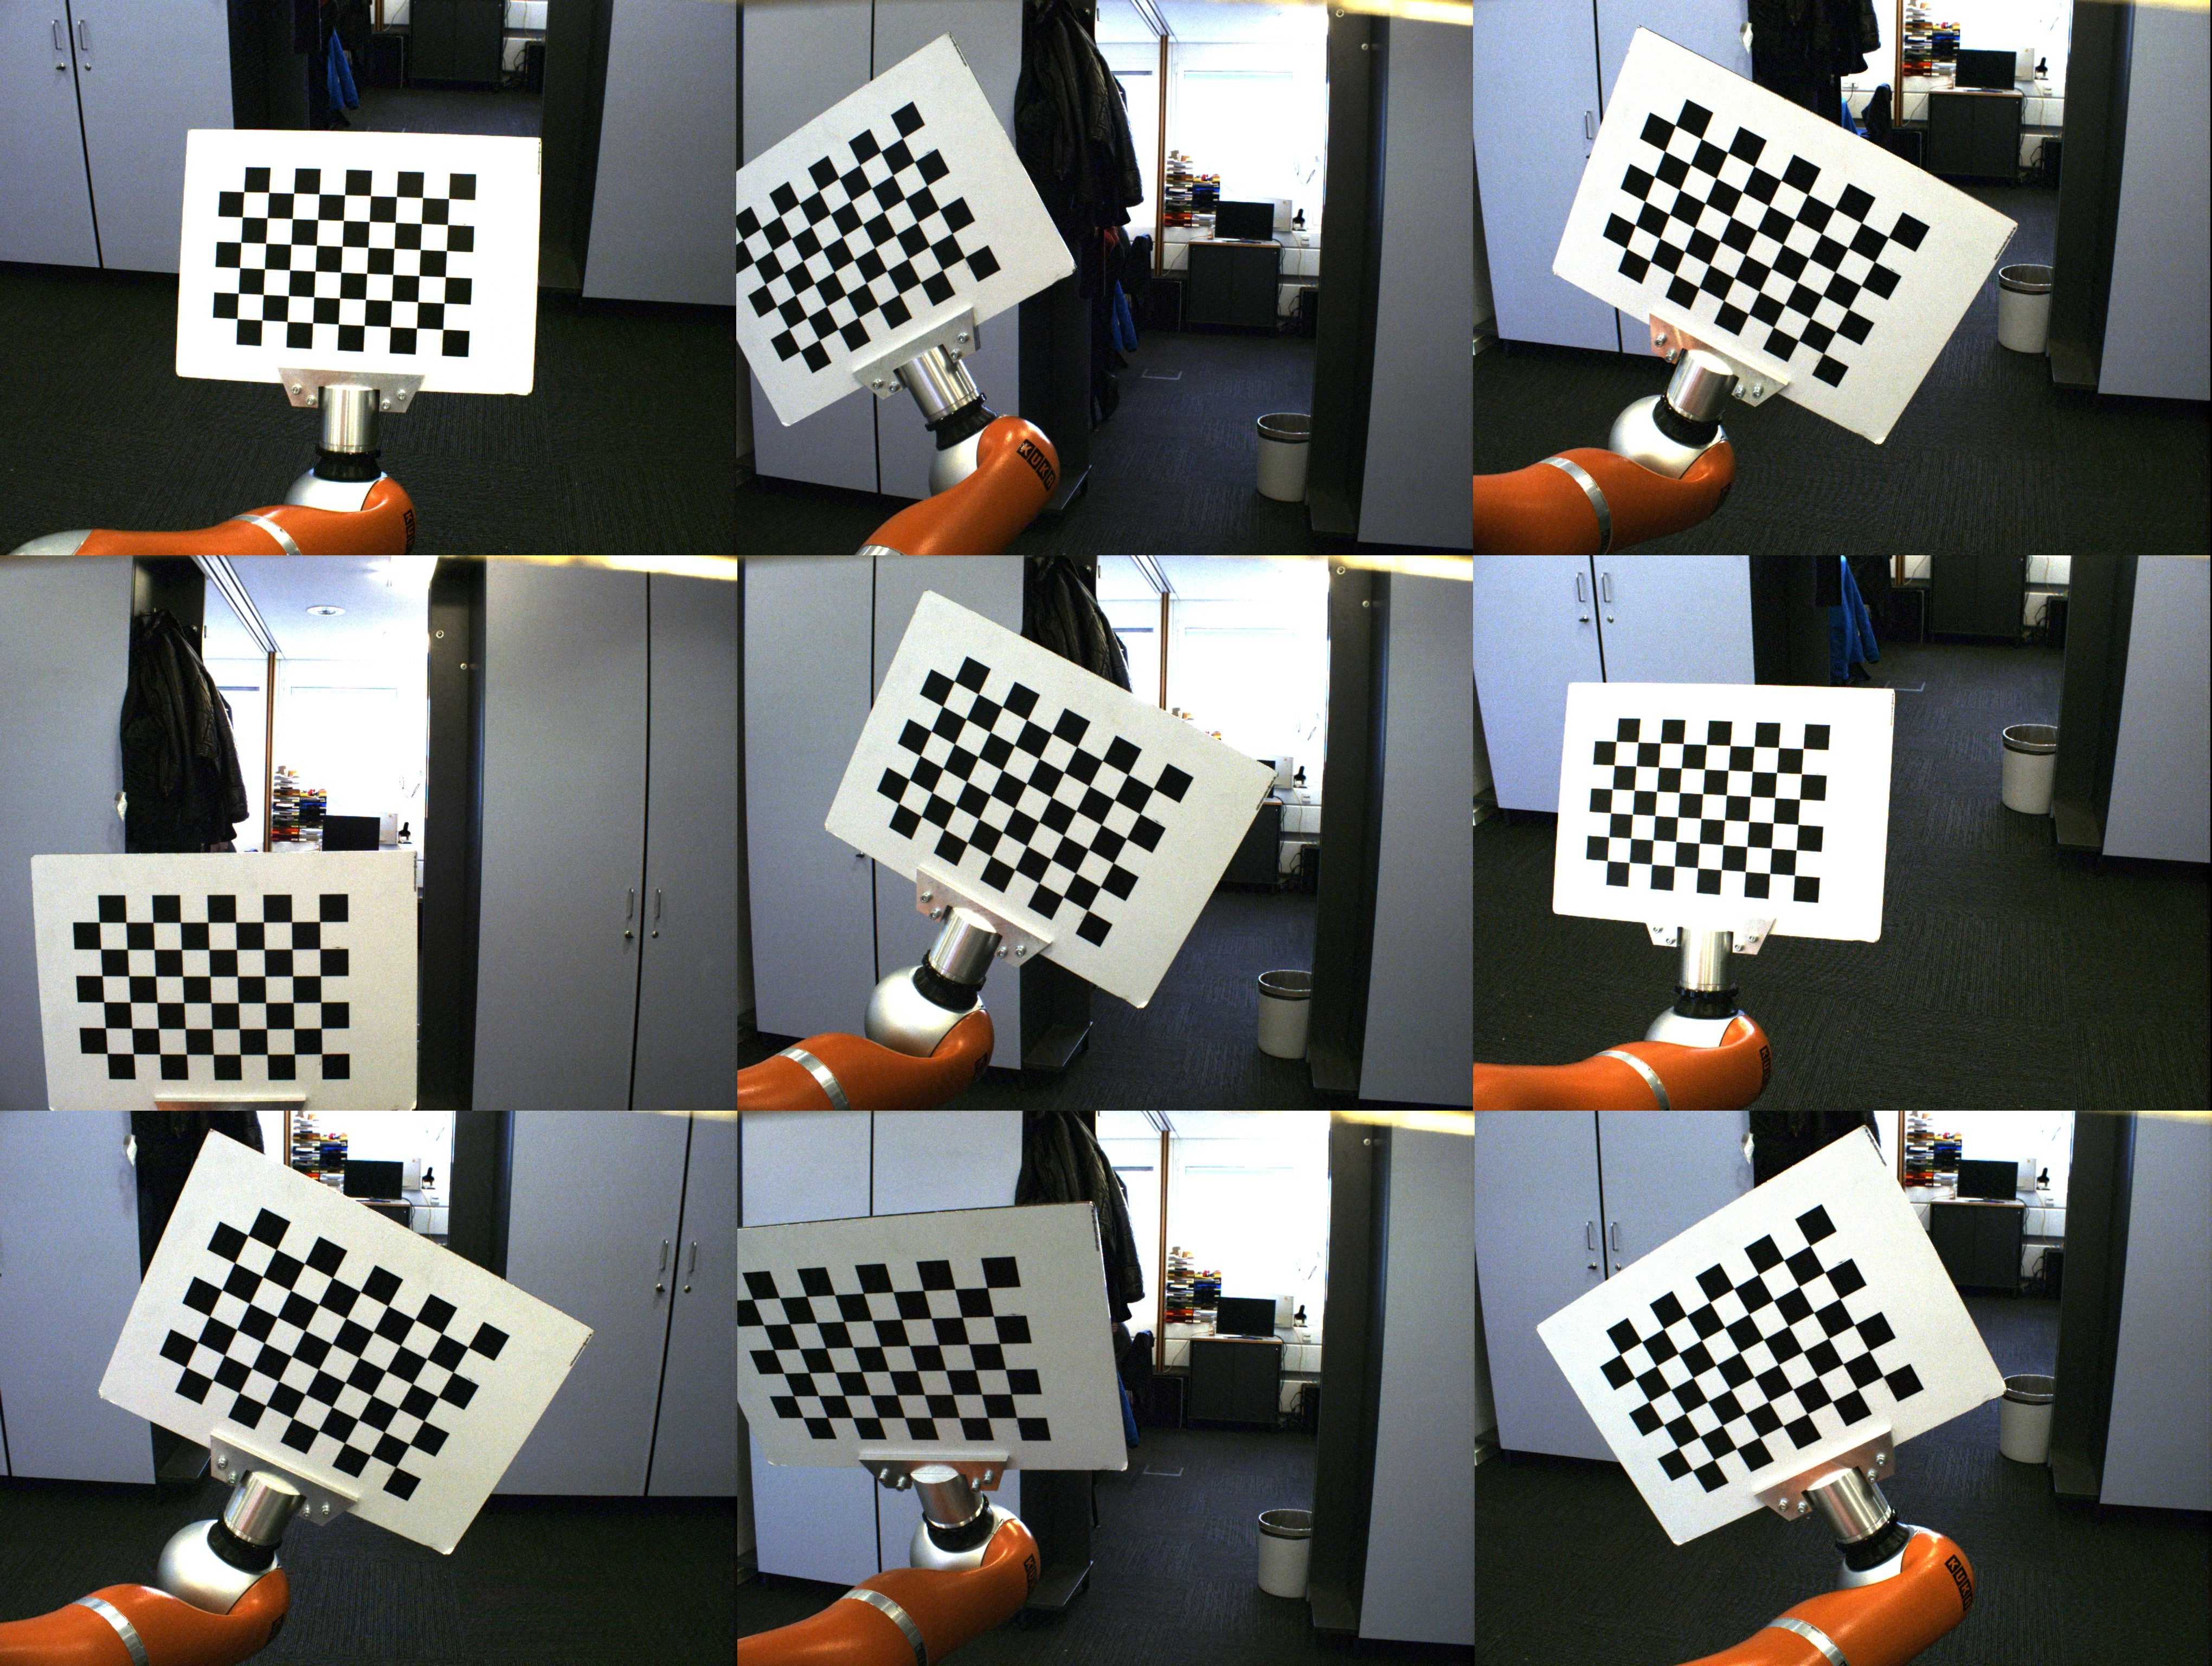
\includegraphics[width=.7\textwidth]{images/calibration_samples}
      \caption{Kalibrierungsbilder}
    \end{figure}
  }

  \onslide<1,3->{
    \begin{center}
      \begin{tikzpicture}[node distance = 2.5em]
        \node(datenaufnahme)[rec]{Datenaufnahme};
          \onslide<3->{ 
        \node (kamerakalibrierung)[rec, below=of datenaufnahme] {Kamerakalibrierung};
        \draw[->] (datenaufnahme) -- (kamerakalibrierung);
      }\onslide<4->{
        \node (datenaufnahme2)[rec, below=of kamerakalibrierung]{Datenaufnahme};
        \draw[<-] (datenaufnahme2) -- (kamerakalibrierung);
      }\onslide<5->{
        \node(kalibrierung) [rec, below=of datenaufnahme2] {Kalibrierung}; 
        \draw[->] (datenaufnahme2) -- (kalibrierung);
      }
    \end{tikzpicture}
  }
\end{center}
\end{frame}
